
\documentclass[preview,border=0.80001bp, convert=imagemagick]{standalone}
%\documentclass{article}
\usepackage{hyperref}
\usepackage{amsmath}
\usepackage{tikz}
\usepackage{miama}
\usepackage{xcolor}
\usepackage[T1]{fontenc}

\newlength\unitlen
\tikzset{
    unit length/.code={\setlength{\unitlen}{#1}},
    unit length = 8pt
}

\begin{document}
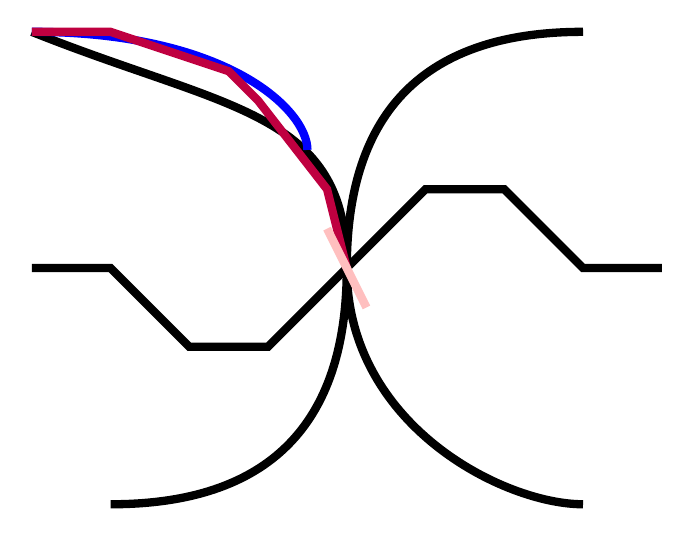
\begin{tikzpicture}[line width=3pt]

        \draw (-4,0) -- (-3,0) -- (-2,-1) -- (-1,-1) -- (1,1) -- (2,1) -- (3,0) -- (4,0);

	% top left to bottom right
	%\draw (-4,3) -- (-2.99,3);
	\draw (-4,3) .. 
	    %controls (-2,3) and (0,2) 
	    controls (-1.5,2) and (0,2) 
	    .. (0,0);

	\draw[color=blue] (-4,3) -- (-3,3);
	\draw[color=blue] (-4,3) ..
	    controls (-1.5, 3) and (-0.5,2)
	.. (-0.5,1.5);

	\draw (0,0) .. 
	    controls (0,-2) and (2,-3) 
	    .. (3,-3);
	%\draw (2.99,-3) -- (4,-3);

	% bottom left to top right
	%\draw (-4,-2.99) -- (-3,-3);
	\draw (-3,-3) .. 
	    controls (-1,-3) and (0,-2) 
	    .. (0,0);
	\draw (0,0) .. 
	    controls (0,2) and (1,3) 
	    .. (3,3);
	%\draw (2.99,3) -- (4,3);


    \draw[color=purple] (-4,3) -- (-3,3) -- (-1.5,2.5) 
	-- (-1.125,2.125) -- (-0.25,1) -- (-0.125, 0.5) -- (0,0)
	;


    \draw[color=pink] (-0.25, 0.5) -- (0.25, -0.5);

\end{tikzpicture}
\end{document}
